\documentclass[a4paper]{article}

\usepackage{mypckg}
\fancypagestyle{ErsteSeite}{%
	\fancyhf{}%
	\setlength\headheight{35pt}
    \fancyhead[R]{\leftmark} %Kopfzeile rechts
    \fancyhead[L]{Compressive Sensing: Basis Pursuit Part II}
    \fancyhead[R]{Arianna Rast}
    \fancyfoot[C]{\thepage}
    }
    
\pagestyle{ErsteSeite}

\begin{document}

\section*{Basis Pursuit Part II}

\subsection*{Review of the null space property and stability}
The basis pursuit the convex relaxation of the \(\ell^0\)-minimization problem, which is NP-hard in general.
The null space property (NSP) of order \(s\) is a necessary and sufficient condition for the exact reconstruction of every \(s\)-sparse vector via the basis pursuit. Here, \enquote{exact reconstruction} means that every vector \(x\in\CC^N\) with at most \(s\) non-zero entries is the unique minimizer of the following optimization problem:
\[
    \min\left\{\|z\|_1\,|\,
    Az=Ax\right\}\,.\]
 Furthermore, one can see that if this is the case, then \(x\) is also the unique minimizer of the corresponding \(\ell^0\)-minimization problem.\\
 The basis pursuit is stable under a sparsity defect in the vector \(x\), if the measurement matrix satisfies the stable null space property (SNSP).

\subsection*{4.3  Robustness}
The goal of this section is to take the noise in the meaasurements into account, additinally to the sparsity defect in the vector \(x\).
More precisely, we want to investigate the following optimization problem, for a given noise level \(\eta\):
\[\min\left\{\|z\|_1\,\big|\,z\in \CC^N,\;\;\|Az-(Ax+e)\|\le \eta\right\}\tag{$P_{1,\eta}$}\,.\]
 For that we need to strengthen the assumptions on the measurement matrix \(A\) to satisfy the robust null space property (RNSP), depending on the \(\ell^q\)-norm, in which the error bound is desired. We start with \(q=1\):
\begin{Def*}
    {Robust null space property}{} A matrix \(A\in\CC^{m\times N}\) is said to satisfy the \emph{robust null space property} with respect to \(\|\cdot\|\) with the constants \(\rho\in (0,1)\) and \(\tau>0\) relative to a set \(S\subseteq[N]\) iff
    \[\forall v\in \CC^N:\;\; \|v_S\|_1\le \rho\|v_{\overline S}\|_1+\tau \|Av\|\,.\tag{RNSP($\|\cdot\|,\rho,\tau,S$)}\]
    \(A \) satisfies the robust null space property of \emph{order} \(s\) with respect to \(\|\cdot\|\) with the constants \(\rho\in (0,1)\) and \(\tau>0\) RNSP(\(\|\cdot\|,\rho,\tau, s\)) iff \(A \) satisfies RNSP(\(\|\cdot\|,\rho,\tau,S\)) for all sets \(S\subseteq[N]\) with \(|S|\le s\).
    \end{Def*}
    We note that the RNSP directly implies the SNSP. The main result is the following theorem.
    \begin{Satz*}
    {(Theorem 4.20 in the book)}{}
    A matrix \(A\in\CC^{m\times N}\) satisfies RNSP(\(\|\cdot\|,\rho,\tau,S\)) if and only if 
    \begin{align*}
    &\forall x,z\in \CC^N:\\ &\|z-x\|_1\le \frac{1+\rho}{1-\rho}(\|z\|_1-\|x\|_1+2\|x_{\overline S}\|_1)+\frac{2\tau}{1-\rho}\|A(x-z)\|\,.
    \end{align*}
    \end{Satz*}
    This is a generalization of the previously discussed theorem for the SNSP (cf. Theorem 4.14 in the book). The following corollary, an \(\ell^1\)-bound for the error, is a key result:
    \begin{Kor*}
        {(Theorem 4.19 in the book)}{}
        Assume that \(A\in\CC^{m\times N}\) satisfies RNSP(\(\|\cdot\|,\rho,\tau,s\)) with \(0<\rho<1\) and \(\tau>0\), \(e\in\CC^m\) with \(\|e\|\le \eta\) and let \(x\in \CC^N\). Then, if \(\mathcal L_{x,\eta}\) is the set of all minimizers of the problem
		\[\min\left\{\|z\|_1\,\big|\,z\in \CC^N,\;\;\|Az-(Ax+e)\|\le \eta\right\}\,,\]
    	then 
        \[\sup_{x^{\#}\in \mathcal L_x}\|x-x^{\#}\|_1\le \frac{2(1+\rho)}{1-\rho}\sigma_s(x)_1+\frac{4\tau}{1-\rho}\eta\,,\]
        i.e. the solution set \(\mathcal L_x\) is contained in a ball of radius \(\frac{2(1+\rho)}{1-\rho}\sigma_s(x)_1+\frac{4\tau}{1-\rho}\eta\) around \(x\) in the \(\ell^1\)-norm, which is small for small \(\eta\) and small sparsity defect \(\sigma_s(x)_1\).
    \end{Kor*}

    Now, let us move on to establish an error bound in \(\ell^q\) for \(q\in [1,\infty)\). We need:
    \begin{Def*}
 {$\ell^q$-robust null space property}{}
 Let \(q\ge 1\). A matrix \(A\in \CC^{m\times N}\) satisfies the \emph{$\ell^q$-robust null space property} of \emph{order} \(s\in \NN\) (with respect to \(\|\cdot\|\)) with the constants \(\rho\in (0,1)\) and \(\tau\ge0\) iff
 \[\forall S\subseteq [N],\;|S|\le s\;\forall v\in \CC^N:\;\;\|v_S\|_q\le \frac{\rho}{s^{1-\frac{1}{q}}}\|v_{\overline S}\|_1+\tau\|Av\|\,.\]
 \end{Def*}
 \begin{Bemerkung*}{}{}
     \begin{itemize}
		\item For \(v\in \CC^N \), \(S\subset [S]\) with \(|S|\le s\) and \(1\le p\le q\), we have 
		\[\|v_S\|_p\le s^{\frac{1}{p}-\frac{1}{q}}\|v_S\|_q\,.\]
		\item Hence, 
		\[
		\ell^q
		\text{-RNSP
		($\|\cdot\|,\rho,\tau,s$)}
		\implies \ell^p \text{-RNSP($s^{\frac{1}{p}-\frac{1}{q}}\|\cdot\|,\rho,\tau,s$)}
		\]
        for \(1\le p\le q\).
		\item In particular, the previously known \(\ell^1\)-RNSP is implied by the \(\ell^q\)-RNSP for \(1\le q<\infty\).
	\end{itemize}
 \end{Bemerkung*}    

 We have the following result:
 \begin{Satz*}
		{(Theorem 4.25 in the book)}{}If a matrix \(A\in \CC^{m\times N}\) satisfies \(\ell^q\)-RNSP($\|\cdot\|,\rho,\tau,s$) for some \(1\le q<\infty\), \(\rho\in (0,1)\), \(\tau>0\), then
		\begin{align*}
			&\forall x,z\in \CC^N,\;\forall p\in [1,q]:\\
			&\|z-x\|_p\le \frac{C}{s^{1-\frac{1}{p}}}(\|z\|_1-\|x\|_1+2\sigma_s(x)_1)+Ds^{\frac{1}{p}-\frac{1}{q}}\|A(x-z)\|\,,\\
		\end{align*}
		where \(C=\frac{(1+\rho)^2}{1-\rho}\) and \(D:=(3+\rho)\tau/(1-\rho)\).
	\end{Satz*}

   The main result is the following corollary of this theorem:
   \begin{Kor*}
		{Robustness of the quadratically constrained basis pursuit}{}
		Assume \(A\in \CC^{m\times N }\) satisfies \(\ell^2 \)-RNSP($\|\cdot\|_2,\rho,\tau, s$) and let \(x\in \CC^N\), \(e\in \CC^m\) with \(\|e\|_2\le \eta\). Then, if \(\mathcal L_{x,\eta}\) is the set of all minimizers of the problem
		\[\min\left\{\|z\|_1\,\big|\,z\in \CC^N,\;\;\|Az-(Ax+e)\|_2\le \eta\right\}\,,\]
		then
		\[\sup_{x^{\#}\in \mathcal L_{x,\eta}}\|x-x^{\#}\|_p\le \frac{C}{s^{1-\frac{1}{p}}}\sigma_s(x)_1+Ds^{\frac{1}{p}-\frac{1}{2}}\eta\]
		for \(p\in [1,2]\) and for some constants \(C,D>0\) that only depend on \(\rho\), \(\tau\).
	\end{Kor*} 
In particular, we receive error bounds in the \(\ell^1\)-norm and the \(\ell^2\)-norm. One can also study the behavior of the error term in \(s\), to see that it decays in the same rate as \(\sigma_s(x)_p\), when the noise \(\eta\) is neglected.

\subsection*{4.4  Recovery of individual vectors}

In this section, we will study a slightly different problem, where we find conditions on the measurement matrix \(A \) and the vector \(x\) such that the basis pursuit recovers \(x\) from the measurements \(Ax\). The difference to the previous section is that we used to have assumptions uniform in \(x\), which then yield the recovery of \emph{all} \(s\)-sparse vectors \(x\). One example is the following theorem: \begin{Satz*}
		{(Theorem 4.26 in the book)}{} Let \(A\in\CC^{m\times N}\) and \(x\in\CC^N\) with support \(S\subseteq[N]\) be given. Then, the following conditions are equivalent:
		\begin{itemize}
			\item[(a)] \(\forall v\in \ker(A)\setminus\{0\}:\;\;|\p{v}{\sgn(x)}|< \|v_{\overline S}\|_1\).
			\item[(b)] \(A_S\) is injective and 
			\[\exists h\in \CC^m:\;\;\left\{\begin{array}{cl}
				(A^*h)_j=\sgn(x_j),&j\in S\;\;\;\text{i.e. }A^*_Sh=\sgn(x_S)\\
				(A^*h)_j<1,&j\in \overline S
			\end{array}\right.\,.\]
			\end{itemize}
			If one (and hence both) of these conditions hold, then \(x\) is the unique minimizer of the problem
			\[\min\left\{\|z\|_1\,\big|\,Az=Ax\right\}\,.\]
	\end{Satz*}

    We see that the condition (a) is related to the NSP in the following way: 
    \[NSP\text{ relative }S\iff \forall x\in \CC^N\te{with }\supp x\subseteq S:\;\;(a)\,.\]
    Condition (b) can be used for the following corollary:

    \begin{Kor*}
			{(Corollary 4.28 in the book)}{}Let \(A=(a_1,\ldots,a_N)\in\CC^{m\times N}\) and \(x\in\CC^N\) with support \(S\subseteq[N]\) be given. Denote \(A_S^{\dagger}=(A^*_SA_S)^{-1}A^*_S\) the left-inverse of \(A_S\). If \(A_S\) is injective and if 
			\begin{align*}
			\forall l\in \overline S:\;\;&\left|\p{A_S^{\dagger}a_l}{\sgn(x_S)}\right|=\left|\p{a_l}{(A_S^{\dagger})^*\sgn(x_S)}\right|\\
			&=\left(A^*(A_S^{\dagger})^*\sgn(x_S)\right)_l<1\,,
			\end{align*}
			then \(x\) is the unique minimizer of the problem
			\[\min\left\{\|z\|_1\,\big|\,Az=Ax\right\}\,.\]
		\end{Kor*}

        The converse this Theorem does not hold in general, as one can see in the following example:
        \[ A=\begin{pmatrix}1&0&-1\\0&1&-1\end{pmatrix}, \;\;x=\begin{pmatrix}\e^{-\pi \I/3}\\\e^{\pi \I/3}\\0\end{pmatrix}\,.\]
		However, if we consider the real problem, the converse does actually hold. The reason for this difference between the complex and the real case is that in the real case, the sign of a vector is a discrete quantity, while in the complex case, it is not.\\
        Another theorem of this type involves the following definition:
        \begin{Def*}
		{}{} Let \(x\in \RR^N \), then the \emph{tangent cone} to the \(\ell^1\)-ball at \(x\) is defined as
		\[T(x)=\mathrm{cone}\left\{z-x\,|\, z\in \RR^N,\;\|z\|_1\le \|x\|_1\right\}=\mathrm{cone}(\overline{B_{\|x\|_1}^{\|\cdot\|_1}(x)})\,.\]
	\end{Def*}
	\vspace{0.5cm}
    \begin{figure}[]
	\begin{minipage}{0.45\linewidth}
	\begin{tikzpicture}[scale=0.8]
		\begin{scope}
			\clip (0,-1) circle (3);
		\fill(0,0) circle (1.5pt);
		\path (0,0) node [below]{$x$};
		\fill[opacity=0.1](1,0)--(0,1)--(-1,0)--(0,-1)--cycle;
		\fill (0,-1) circle (1.5pt);
		\path (0,-1) node [below]{$0$};
		\fill[opacity=0.2] (0,-1)--(4,3)--(0,4)--(-4,3)--cycle;
		\end{scope}
		\end{tikzpicture}
	\end{minipage}
	\begin{minipage}{0.45\linewidth}
		\centering
	\begin{tikzpicture}[scale=0.8]
		\begin{scope}
			\clip (0,-1) circle (3);
		\fill(0,0) circle (1.5pt);
		\path (0,0) node [below]{$x$};
		\fill[opacity=0.1](1,0)--(0,1)--(-1,0)--(0,-1)--cycle;
		\fill (-0.75,-0.25) circle (1.5pt);
		\path (-0.75,-0.25) node [below]{$0$};
		\fill[opacity=0.2] (-4,3)--(4,-5)--(8,-1)--(0,7)--cycle;
		\end{scope}
		\end{tikzpicture}
	\end{minipage}
    \caption{The tangent cone to the \(\ell^1\)-ball in \(\RR^2\) is either a cone with \(90^{\circ}\) (left) or \(180^{\circ}\) (right) opening angle, depending on the position of the point \(0\) in the \(\ell^1\)-ball.}
\end{figure}

The exact reconstruction of \(x\) is then characterized by:
\begin{Satz*}
	{(Theorem 4.35 in the book)}{} Let \(A\in \RR^{m\times N }\) and \(x\in \RR^N \). Then
	\[
	\left.\begin{array}{c}

		x\text{ is the unique minimizer} \\  \text{of }
		\left\{\|z\|_1\,\big|\, Az=Ax\right\}
	\end{array}\right\} \iff \ker(A)\cap T(x)=\{0\}\,.
	\]
\end{Satz*}

Furthermore, this characterization is robust under noise in the measurements in the following sense:
\begin{Satz*}
{(Theorem 4.36 in the book)}{} Let \(A\in \RR^{m\times N}\), \(x\in \RR^N\) and \(e\in \RR^m \) such that \(\|e\|_2\le \eta\). Assume
\[\exists \tau>0:\;\;\inf_{v\in T(x)\cap \pp B_1^{\|\cdot\|_2}}\|Av\|_2\ge \tau\,.\]
Then, if \(x^{\#}\) is a minimizer of the problem
\[\min\left\{\|z\|_1\,\big|\,z\in \RR^N,\;\;\|Az-(Ax+e)\|_2\le \eta\right\}\,,\]
we have that
\[\|x-x^{\#}\|_2\le \frac{2\eta}{\tau}\,.\]
	\end{Satz*}	

    
 \end{document} 
